\documentclass [a4paper,11pt]{article}
\usepackage{amssymb}
\usepackage{amsthm}
\usepackage[intlimits]{amsmath}
\usepackage[polish]{babel}
\usepackage[utf8]{inputenc}
\usepackage[T1]{fontenc}
\frenchspacing
\usepackage{indentfirst}
\usepackage{graphicx}
\usepackage{subfig}
\usepackage{mathptmx}
\usepackage{geometry}
\usepackage{wrapfig}
\usepackage{enumitem}
\usepackage{tabularx}

\title{Moduł Younga}
\author{Pęcak Tomasz, Bielech Maciej}

\begin{document}
	
	\renewcommand*{\figurename}{Tabela} 
	\newgeometry{tmargin=2cm, bmargin=2cm, lmargin=2cm, rmargin=2cm}
	
	\linespread{1.5}
	\selectfont

	\begin{table}[]
		\centering
		\begin{tabular}{lllllll}
			\cline{1-6}
			\multicolumn{1}{|c|}{\begin{tabular}[c]{@{}c@{}}EAiIB\\ Informatyka\end{tabular}} & \multicolumn{2}{l|}{\begin{tabular}[c]{@{}l@{}}Pęcak Tomasz\\ Bielech Maciej\end{tabular}} & \multicolumn{1}{c|}{\begin{tabular}[c]{@{}c@{}}Rok\\ II\end{tabular}} & \multicolumn{1}{c|}{\begin{tabular}[c]{@{}c@{}}Grupa\\ 3a\end{tabular}} & \multicolumn{1}{c|}{\begin{tabular}[c]{@{}c@{}}Zespół\\ II\end{tabular}} &  \\ \cline{1-6}
			\multicolumn{1}{|c|}{\begin{tabular}[c]{@{}c@{}}Pracownia\\ FIZYCZNA\\ WFiIS AGH\end{tabular}} & \multicolumn{4}{l|}{\begin{tabular}[c]{@{}l@{}}Temat:\\ \textbf{Fale podłużne w ciałach stałych } \end{tabular}} & 
			\multicolumn{1}{l|}{\begin{tabular}[c]{@{}l@{}}nr ćwiczenia:\\ 29\end{tabular}} &  \\ \cline{1-6}
			\multicolumn{1}{|l|}{\begin{tabular}[c]{@{}c@{}}Data wykonania:\\ 28.10.2017\end{tabular}} & \multicolumn{1}{c|}{\begin{tabular}[c]{@{}c@{}}Data oddania:\\ 31.10.2017\end{tabular}} & \multicolumn{1}{l|}{\begin{tabular}[c]{@{}l@{}}Zwrot do poprawki:\\ \phantom{data poprawki}\end{tabular}} & \multicolumn{1}{l|}{\begin{tabular}[c]{@{}l@{}}Data oddania:\\  \phantom{data oddania}\end{tabular}} & \multicolumn{1}{l|}{\begin{tabular}[c]{@{}l@{}}Data zaliczenia:\\  \phantom{data zaliczenia}\end{tabular}} & \multicolumn{1}{l|}{\begin{tabular}[c]{@{}l@{}}OCENA:\\ \phantom{ocena}\end{tabular}} &  \\ \cline{1-6} 
		\end{tabular}
	\end{table}
	 \hspace{5mm}

	\section{Wstęp}
	Celem ćwiczenia było wyznaczenie wartości modułu Younga dla różnych materiałów przy wykorzystaniu rónania fali rozchodzącej się w pręcie. 
	
	\begin{equation}
	\label{eq:prawohooka}
	\Delta l=\frac{Fl}{SE}.
	\end{equation}
	\begin{equation}
	\label{eq:modulYounga}
	E=\frac{\sigma}{\epsilon}.
	\end{equation}

	\renewcommand*{\figurename}{Wykres} 
	\setcounter{figure}{0}
	\begin{figure}[!h]
		\begin{center}
		
		\end{center}
		\caption{Charakterystyka Modułu Younga. Źródło: pl.wikipedia.org}
		\label{fig:wykMod}
	\end{figure}
	
	\begin{equation}
	\label{eq:wzorroboczy}
	E = \frac{4l}{\pi d^2 a} \text{.}
	\end{equation}
	
	Wartość współczynnika \textit{a} oraz jego niepewność \textit{u(a)} wyznaczymy korzystając z regresji liniowej.
	\section{Wykonanie ćwiczenia}
	Ćwiczenie wykonywaliśmy dla drutów: mosiężnego, stalowego, miedzianego i aluminiowego. Dla każdego z nich wykonaliśmy nastepujące czynności:
	\begin{itemize}
		\item W pierwszym kroku dokonaliśmy pomiaru wymiarów próbki danego materiału w celu wyznaczenia jego objętości. W zależności od kształtu stosowaliśmy: taśmę mierniczą o dokładności $\pm1$ mm lub suwmiarkę $\pm0.05$ mm.
		\item Następnie każdą próbkę zwarzyliśmy. Ze względu na różne wielkośc próbek używaliśmy wag o różnych dokładnościach( $\pm1$g lub $\pm0.001$g).
		
		\item W kolejnym kroku zmierzyliśmy długość pręta przy pomocy taśmy mierniczej.
		
		\item Na końcu dokonaliśmy pomiaru częstotliwości harmoniczych przy pomocy oscyloskopu w programie Zelscope. W tym celu umieśliśmy pręt na nitkach stojaka, by mógł swobonie drgać. Ustawiliśmy mikrofon w odpowiedniej odległości od drutu. Następnie uderzaliśmy młotkiem w koniec pręta i zapisywaliśmy wyniki uzykane w programie.  
	\end{itemize}

	\renewcommand*{\figurename}{Tabela} 
	\setcounter{figure}{0}
	\begin{figure}[!h]
		\centering
		\caption{Pomiary dla materiału miedzianego.}
		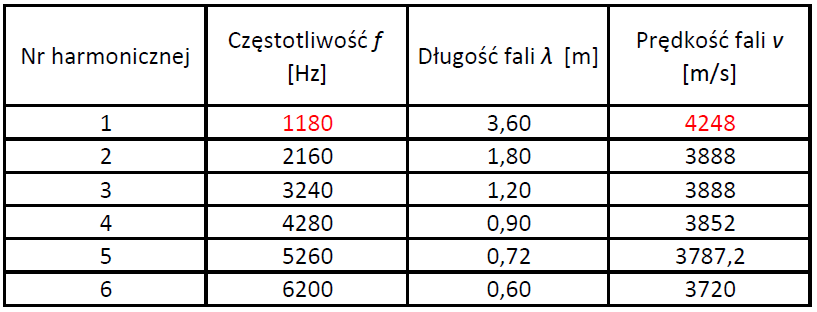
\includegraphics[width=0.7\textwidth]{tabmiedz}
		\label{fig:tabmiedz}
	\end{figure}
	\begin{figure}[!h]
		\centering
		\caption{Pomiary dla materiału aluminiowego.}
		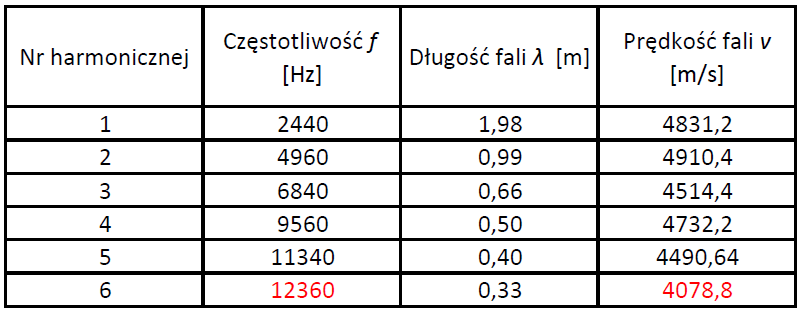
\includegraphics[width=0.7\textwidth]{tabaluminium}
		\label{fig:tabaluminium}
	\end{figure}
	\begin{figure}[!h]
		\centering
		\caption{Pomiary dla materiału mosiężnego.}
		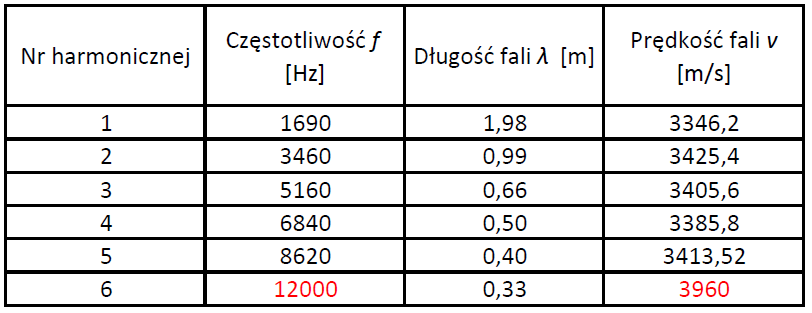
\includegraphics[width=0.7\textwidth]{tabmosiadz}
		\label{fig:tabmosiadz}
	\end{figure}
	\begin{figure}[!h]
		\centering
		\caption{Pomiary dla materiału stalowego.}
		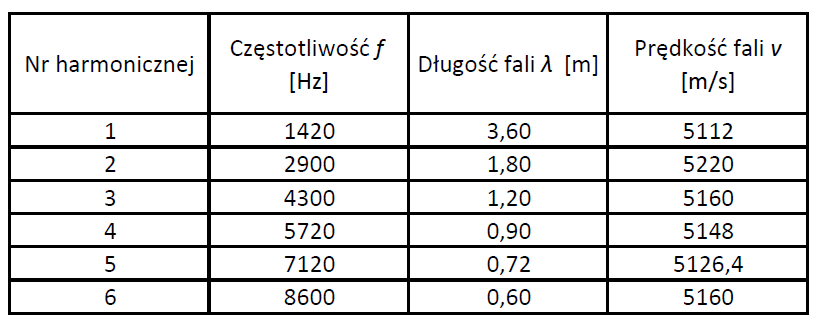
\includegraphics[width=0.7\textwidth]{tabstal}
		\label{fig:tabstal}
	\end{figure}

	\section{Opracowanie danych pomiarowych}\label{sec:opr}
	\subsection{Pomiary i ich niepewności.}
		
		Wszystkie wielkości mierzyliśmy niewielką ilość razy, dlatego dla każdej z nich przyjmujemy ocenę niepewności typu B, co w naszym przypadku będzie odpowiadać dokładności przyrządu pomiarowego.\newline
		W każdym przypadku $u(\lambda) = u(l) $ oraz $u(f) = 20 \text{ Hz}$.
		\begin{table}[h!]
			\centering
			\caption{Niepewności standardowe miedzi}
			\label{tab:nsmiedz}
			\begin{tabular}{l|l|l|l|l|l}
				 Symbol & \textit{$d$} [mm]  & \textit{$d_w$} [mm]   & \textit{$l$} [mm]     &  \textit{$m$} [g]  \\ \hline
				 Wartość(niepewność) & 15,2(5)      & 17,95(5) & 1801(1) & 761(1) \\
			\end{tabular}
		\end{table}
	
		\begin{table}[h!]
			\centering
			\caption{Niepewności standardowe aluminium}
			\label{tab:nsaluminium}
			\begin{tabular}{l|l|l|l|l}
				Symbol & \textit{$h$} [mm]  & \textit{$d$} [mm]   & \textit{$l$} [mm]     &  \textit{$m$} [g]   \\ \hline
				Wartość(niepewność) & 43,9(5)      & 4,9(5) & 999(1) & 23,891(1) \\
			\end{tabular}
		\end{table}
		
		\begin{table}[h!]
			\centering
			\caption{Niepewności standardowe stal}
			\label{tab:nsstal}
			\begin{tabular}{l|l|l|l|l|l}
				Symbol & \textit{$h$} [mm]  & \textit{$b$} [mm]   & \textit{$c$} [mm]  & \textit{$b$} [mm]      & \textit{$m$} [g]   \\ \hline
				Wartość(niepewność) &19,80(5) & 14,05(5)      & 14,20(5) & 1800(1) & 30,861(1) \\
			\end{tabular}
		\end{table}
	
		\begin{table}[h!]
			\centering
			\caption{Niepewności standardowe mosiadz}
			\label{tab:nsmosiadz}
			\begin{tabular}{l|l|l|l|l}
					Symbol & \textit{$d$} [mm]  & \textit{$h$} [mm]   & \textit{$l$} [mm]     & \textit{$m$} [g]   \\ \hline
				Wartość(niepewność)	& 5,90(5)      & 31,10(5) & 1800(1) & 74(1) \\
			\end{tabular}
		\end{table}
	Niepewność złożona powierzchni prostokąta:
		\begin{equation}
		u(P_P)=\sqrt{\bigg(\frac{\partial P_P}{\partial b}u(b)\bigg)^2 + \bigg(\frac{\partial P_p}{\partial a}u(a)\bigg)^2} = \sqrt{\bigg(bu(a)\bigg)^2+\bigg(au(b) \bigg)^2}
			\end{equation}
			
	Niepewność złożona powierzchni koła:
		\begin{equation}
		u(V)=\sqrt{\bigg(\frac{\partial P_P}{\partial d}u(d)\bigg)^2} = \sqrt{\bigg(\frac{\pi}{2}du(d)\bigg)^2}
		\end{equation}
		
	Niepewność złożona objętości:
	\begin{equation}
	u(V)=\sqrt{\bigg(\frac{\partial V}{\partial h}u(h)\bigg)^2 + \bigg(\frac{\partial V}{\partial P_p}u(P_p)\bigg)^2} = \sqrt{\bigg(hu(P_p)\bigg)^2+\bigg(P_pu(h) \bigg)^2}
	\end{equation}
	
	Niepewność złożona gęstości:
	\begin{equation}
	u(\rho)=\sqrt{\bigg(\frac{\partial \rho}{\partial V}u(V)\bigg)^2+\bigg(\frac{\partial \rho}{\partial \lambda}u(\lambda)\bigg)^2}=\sqrt{\bigg(-\frac{m}{V^2}u(V)\bigg)^2+\bigg(\frac{1}{V}u(m) \bigg)^2}
	\end{equation}
	
	Niepewność złożona prędkości:
	\begin{equation}
	u(v)=\sqrt{\bigg(\frac{\partial v}{\partial f}u(f)\bigg)^2+\bigg(\frac{\partial v}{\partial \lambda}u(\lambda)\bigg)^2}=\sqrt{\bigg(\lambda u(f)\bigg)^2+\bigg(f u(\lambda)\bigg)^2}
	\end{equation}
	
	Niepewność złożona modułu Younga:
	\begin{equation}
			 u(E)=\sqrt{\bigg(\frac{\partial E}{\partial \rho}u(\rho)\bigg)^2+\bigg(\frac{\partial E}{\partial v}u(v)\bigg)^2} =
	\sqrt{\bigg(v^2 u(\rho)\bigg)^2+\bigg(2 \rho v u(v)\bigg)^2}
	\end{equation}


	
	\subsection{Opracowanie danych dla drutu mosiężnego.}\label{sec:drm}
	\renewcommand*{\figurename}{Wykres} 
	\setcounter{figure}{1}
	\begin{figure}[!h]
		\centering

		\caption{Wykres zależności wydłużenia od siły dla drutu mosiężnego.}
		\label{fig:wykmosiadz}
	\end{figure}

	\begin{enumerate}[label=\alph*)]
		
		\item Analiza błędów.
		
		Nie stwierdziliśmy wystąpienia błędów grubych, gdyż na wykresie (\ref{fig:wykmosiadz}) nie zauważamy pomiarów odstających.
		
		\item Prawo przenoszenia niepewności.
		
		Wykorzystując regresję liniową, obliczamy wartość współczynnika $a$ prostej i  jej dokładność $u(a)$:
		\begin{align}
		a = 1,86 \cdot 10^{-5} \text{ }\mathrm{\frac{m}{N}},\label{a} \\
		u(a) = 3,91 \cdot 10^{-7} \text{ }\mathrm{\frac{m}{N}},
		\end{align}
		Następnie wyznaczamy moduł Younga ze wzoru roboczego (\ref{eq:wzorroboczy}).
		$$ E = 124 \text{ GPa} $$
		Obliczając niepewność złożoną (\ref{eq:niepewnosczlozonamosiadz}) oraz rozszerzoną (\ref{eq:rozszerzonamosiadz}) dochodzimy do wyników: 
		\begin{equation}
		\label{eq:niepewnosczlozonamosiadz}
		u_c(E) = \sqrt{ \left[ \frac{4}{\pi d^2a}u(l) \right]^2 + \left[ -\frac{8l}{\pi d^3 a}u(d) \right]^2 + \left[ -\frac{4l}{\pi d^2 a^2}u(a) \right]^2}
		\end{equation}
		$$ u_c(E) = 4,13 \text{ GPa,} $$
		\begin{equation}
		\label{eq:rozszerzonamosiadz}
		U(E) = k\cdot u_c(E)
		\end{equation}
		$$ U(E) = 2 \cdot 4,13 \text{ }\mathrm{GPa} = 8,26 \text{ }\mathrm{GPa} $$
		
		Niepewość względna złożona (\ref{eq:niepewnosczlozonawzglmosiadz}) jest równa:
		\begin{equation}
		\label{eq:niepewnosczlozonawzglmosiadz}
		\frac{u_c(E)}{E} = \sqrt{ \left[ \frac{u(l)}{l} \right]^2 + \left[ -2\frac{u(d)}{d} \right]^2 + \left[ -\frac{u(a)}{a} \right]^2}
		\end{equation}
		$$ \frac{u_c(E)}{E} = 3,34\% $$
		
		\item Zastosowanie niepewności rozszerzonej do oceny zgodności z wartością dokładną.
		
		Różnica pomiedzy obliczoną wartością modułu Younga ($E=123,58  \text{ }\mathrm{GPa}$), a wartością tabelaryczną wynosi:
		\begin{equation}
		\label{eq:roznicamosiadz}
		|E - E_0| = \left|124 \text{ }\mathrm{GPa} - 100 \text{ }\mathrm{GPa}\right| = 24 \text{ }\mathrm{GPa}.
		\end{equation}
		$$
		|E - E_0| > U(E)
		$$
		Wyniki pomiarów w przybliżeniu liniowe i niezgodny wynik mogą świadczyć o błędzie systematycznym. Było to złe wyzerowanie czujnika, dlatego każdy z pomiarów wskazuje niższą wartość wydłużenia drutu niż spodziewana. Błąd ten zauważyliśmy podczas wstępnej analizy pomiarów, dlatego wykonaliśmy kolejną serię pomiarów dla drutu mosiężnego.
	\end{enumerate}

	\subsection{Opracowanie danych dla drutu mosiężnego. Wyniki drugiej serii pomiarów.}
	
	\begin{figure}[!h]
		\centering

		\caption{Wykres zależności wydłużenia od siły dla drugiej serii pomiarów drutu mosiężnego.}
		\label{fig:wykmosiadz2}
	\end{figure}
	
	\begin{enumerate}[label=\alph*)]
		\item Analiza błędów.
		
		Nie stwierdziliśmy wystąpienia błędów grubych, gdyż na wykresie (\ref{fig:wykmosiadz2}) nie zauważamy pomiarów odstających.
		
		\item Prawo przenoszenia niepewności.
		
		Analogicznie jak w podsekcji \ref{sec:drm} wyznaczamy współczynnik $a$ i wartość modułu Younga:
		\begin{align}
		a = 2,00 \cdot 10^{-5} \text{ }\mathrm{\frac{m}{N}},\label{a} \\
		u(a) = 3,50 \cdot 10^{-7} \text{ }\mathrm{\frac{m}{N}},
		\end{align}
		$$ E = 116 \text{ GPa} $$
		Obliczając niepewność (\ref{eq:niepewnosczlozonamosiadz}) oraz rozszerzoną (\ref{eq:rozszerzonamosiadz}) dochodzimy do wyników: 
		$$ u_c(E) = 3,01 \text{ GPa,} $$
		$$ U(E) = 2 \cdot 3,01 \text{ }\mathrm{GPa} = 6,02 \text{ }\mathrm{GPa} $$
		
		Niepewość względna złożona (\ref{eq:niepewnosczlozonawzglmosiadz}) jest równa:
		$$ \frac{u_c(E)}{E} = 2,6\% $$
		
		\item Zastosowanie niepewności rozszerzonej do oceny zgodności z wartością dokładną.
		
		Różnica pomiedzy obliczoną wartością modułu Younga ($E=116  \text{ }\mathrm{GPa}$), a wartością tabelaryczną wynosi:
		\begin{equation}
		\label{eq:roznicamosiadz2}
		|E - E_0| = \left|116 \text{ }\mathrm{GPa} - 100 \text{ }\mathrm{GPa}\right| = 16 \text{ }\mathrm{GPa}.
		\end{equation}
		$$
		|E - E_0| > U(E)
		$$
		
		
	\end{enumerate}

	\subsection{Opracowanie danych dla drutu stalowego.}
	\begin{figure}[!h]
		\centering
%		\includegraphics[width=0.8\textwidth]{}
		\caption{Wykres zależności wydłużenia od siły dla drutu stalowego.}
		\label{fig:wykstal}
	\end{figure}
	
	\begin{enumerate}[label=\alph*)]
		\item Analiza błędów.
		
		Stwierdziliśmy wystąpienie dwóch pomiarów odstających, które możemy utożsamiać z błędami grubymi. Błędy te zaznaczylismy na wykresie (\ref{fig:wykstal}). Mogły one zostać spowodowane niewystarczającym wydłużeniem dla pierwszego pomiaru, a dla ostatniego pomiaru zbyt dużym naprężeniem, zbliżonym do granicy sprężystości, lub błędnym odczytem pomiaru z czujnika.
		
		\item Prawo przenoszenia niepewności.
		
		Podobnie jak dla drutu mosiężnego w podsekcji \ref{sec:drm} wyznaczamy współczynnik $a$ i wartość modułu Younga:
		\begin{align}
		a = 1,60 \cdot 10^{-5} \text{ }\mathrm{\frac{m}{N}},\label{a} \\
		u(a) = 4,55 \cdot 10^{-7} \text{ }\mathrm{\frac{m}{N}},
		\end{align}
		$$ E = 176 \text{ GPa} $$
		Obliczając niepewność złożoną (\ref{eq:niepewnosczlozonamosiadz}) oraz rozszerzoną (\ref{eq:rozszerzonamosiadz}) dochodzimy do wyników: 
		$$ u_c(E) = 7,13 \text{ GPa,} $$
		$$ U(E) = 2 \cdot 7,13 \text{ }\mathrm{GPa} = 14,26 \text{ }\mathrm{GPa} $$
		
		Niepewość względna złożona jest równa:
		$$ \frac{u_c(E)}{E} = 4,03\% $$
		
		\item Zastosowanie niepewności rozszerzonej do oceny zgodności z wartością dokładną.
		
		Różnica pomiedzy obliczoną wartością modułu Younga ($E=176,47  \text{ }\mathrm{GPa}$), a wartością tabelaryczną wynosi:
		\begin{equation}
		\label{eq:roznicastal}
		|E - E_0| = \left|176 \text{ }\mathrm{GPa} - 215 \text{ }\mathrm{GPa}\right| = 39 \text{ }\mathrm{GPa}.
		\end{equation}
		$$
		|E - E_0| > U(E)
		$$
		
		
	\end{enumerate}
	
	
	
	\section{Podsumowanie}
	\begin{center}
		\begin{tabular}{|c|c|c|c|c|c|c|}
			\hline Opis wielkości & $ E_0 \left[ \text{GPa} \right]$ & $E \left[ \text{GPa} \right]$ & $U(E) \left[ \text{GPa} \right]$ & $ \frac{u(E)}{E} $& $(0,9E_0-U(E); 1,1E_0 + U(E))$\\
			\hline Pomiary drutu mosiężnego I & 100 & 124 & 8 & 3,34 \% & (82 ;118) \\
			\hline Pomiary drutu mosiężnego II & 100 & 116 & 6 & 2,6 \% & (84 ; 116) \\  
			\hline Pomiary drutu stalowego & 210-220 & 176  & 14 &  4,03 \% & (175 ; 256)\\ 
			\hline 
		\end{tabular} 
	\end{center}
\vspace{1em}

\begin{itemize}
	\item Określenie poprawności wyników naszych doświadczeń jest trudne, ponieważ nie da się jednoznacznie określić wartości tabelarycznej dla danego metalu. Wynika to z nieznajomości dokładnego składu metalu (stopu), a także ze zużycia drutu. W naszych badaniach przyjmujemy rozrzut rzędu $\pm10\%$ dla wartości odczytanych z tabel fizycznych.
	
	\item Zarówno dla pierwszych jak i drugich pomiarów dla mosiądzu obliczona wartość modułu wykracza poza przedział ($E_0-U(E), E_0+U(E)$). Po uwzględnieniu dziesięcioprocentowego rozrzutu drugą serię pomiarów możemy uznać za poprawną w zakresie wyznaczonej niepewności. Pierwsza seria pomiarów nadal daje wynik niepoprawny, co potwierdza nasze obawy co do błędu systematycznego.
	
	\item Podobnie jak w przypadku drugiej serii pomiarów dla mosiądzu wartość modułu Younga dla stali wykracza poza $E_0 \pm U(E)$, lecz po uwzględnieniu dziesięcioprocentowego rozrzutu od wartości tablicowej możemy uznać obliczoną wartość za poprawną w zakresie wyznaczonej niepewności.
	
\end{itemize}

\end{document}